\chapter{Common Analysis Items}
\label{chapter:common_analysis_objects}

%todo fill in the citations
After the collisions and interactions in the LHC, final state particles leave their mark on various detector components as electronic signal. These electronic signal are saved in hard disks and tapes. It takes various steps of reconstruction identification, cleaning and calibration before the raw electronic information becomes analysis-ready physics objects. The different particle signatures left on the detector can help
with their identifications. Figure~\ref{fig:particleSignature} shows the different signature that different particles leave on the ATLAS detector.

In this chapter, different analysis final state objects are described. In Section~\ref{sec:Tracks}, detector tracks and vertex construction is covered. In Section~\ref{sec:Muon}, Section~\ref{sec:Jet} and Section~\ref{sec:Photon}, the formation of muons, jets and photons from detector signal
through their reconstruction, identification, isolation as well as calibration are discussed in detail. 

\begin{figure}[!htb]
    \begin{center}
        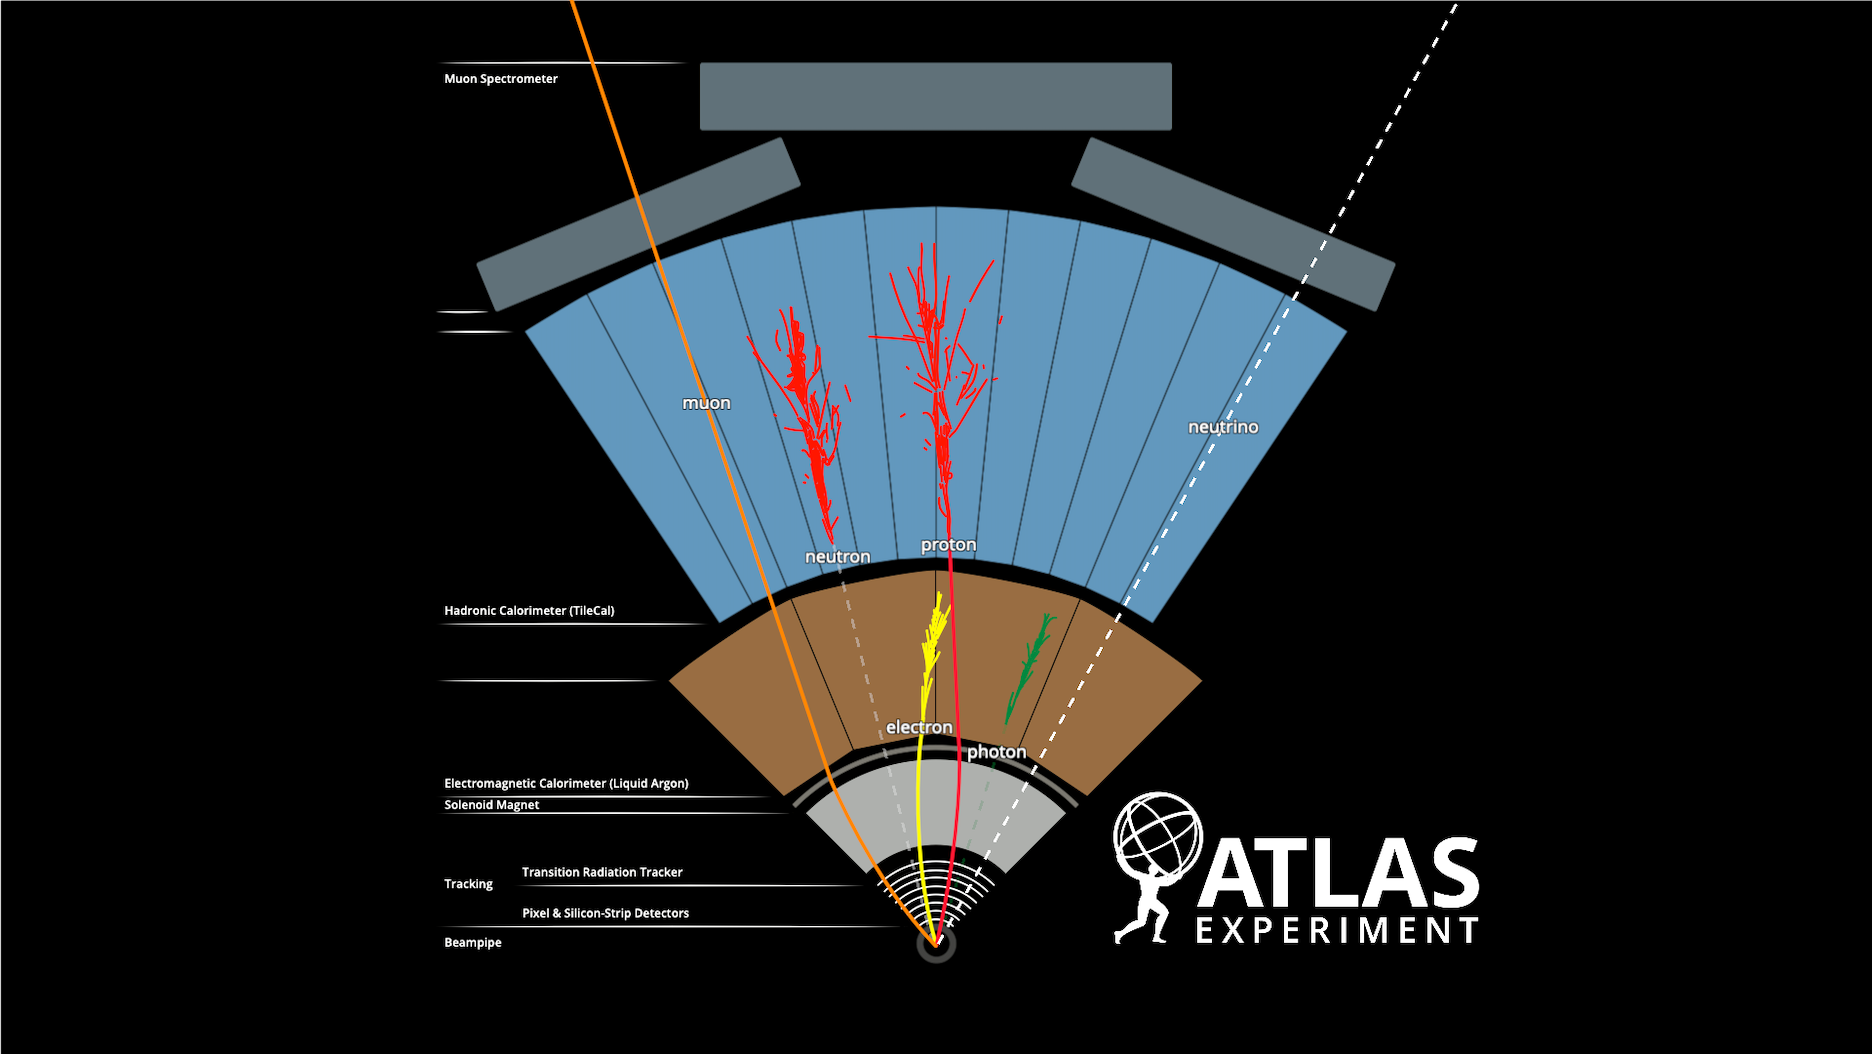
\includegraphics[width=1.1\textwidth]{figures/common_ana/ParticleSignature}
        \caption{        
            Different particles displays a different particle signature characteristics in the ATLAS detector~\cite{Mehlhase:2770815}. The different characteristics can then be used to identify and reconstruct the objects from one another. 
        }
        \label{fig:particleSignature}
    \end{center}
\end{figure}

\section{Tracks and vertices}
\label{sec:Tracks}
Charged particles leave trajectories in two distinct ATLAS sub-detector systems, namely the inner detector(ID) and the muon system(MS). Details regarding the subdetector system can be found in Chapter~\ref{chapter:ATLAS}.

\subsection{ID Tracks}
To reconstruct a track from detector raw hit information, coincidence measurements in multiple layers are first used to find a track seed. Then, a Kalman-filter is used to fit the tracks~\cite{track}, irrelevant hits from pile-up~\footnote{Pile-ups are hits and tracks that result from multiple collisions other than the primary collision. } are removed through the filter. Figure~\ref{fig:track} shows a schematic diagram for a track.

\begin{figure}[!htb]
    \begin{center}
        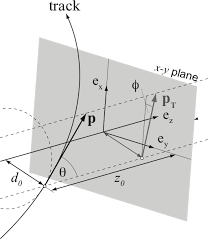
\includegraphics[width=0.3\textwidth]{figures/common_ana/Track}
        \caption{ 
        Schematic view of how the parameters associated with track creation in ATLAS.
        }
        \label{fig:track}
    \end{center}
\end{figure}

\subsection{Vertices}
Once tracks are formed in the inner detector, primary vertices can be constructed from the track directions and their intersection points. Vertexing picks out tracks and hits that are associated with a single interaction. It is helpful in discriminating event-of-interest tracks from pile-up tracks. Effective vertexing is of great importance to event reconstruction, especially in more recent LHC runs, where the higher luminosity has resulted in additional in-time and out-of-time pile-ups.

\begin{figure}[!htb]
    \begin{center}
        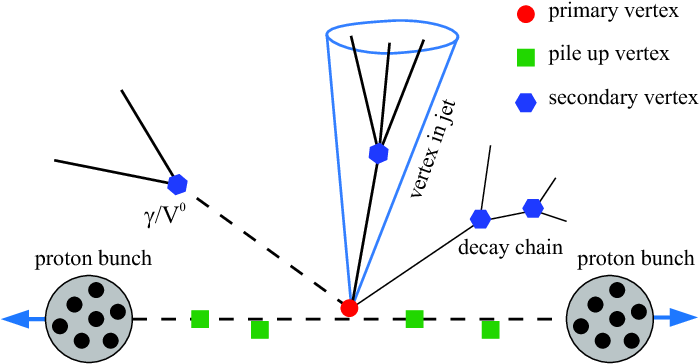
\includegraphics[width=0.4\textwidth]{figures/common_ana/Vertex}
        \caption{        
            Schematic view showing vertexing in ATLAS\cite{4774734}.
        }
    \end{center}
\end{figure}

Vertexing consists of a couple of different steps: First, a vertex seed is found by filtering the points where most interactions are found. Then, tracks consistent with the chosen vertex seed are put into a group. After that, the vertex position and the associated error of the vertex is found by an adaptive vertex fitting algorithm~\cite{track}. Lastly, the unused tracks are used for the next vertex creation. The process then repeats until no tracks remain. 

The vertex with the highest $P_{T}$ particles originated from it is considered the hard-primary vertex of the event, the others are considered the pile-up primary vertices. Somtimes particles produced from the primary vertex decays further, the interaction points where the further decay occur are known as the secondary vertices.

Particle formation from detector hit information in the following sections relies on the tracks and primary vertex reconstruction above.

\section{Muons}
\label{sec:Muon}
Muons in ATLAS are formed from both the tracks and primary vertex information described in the above section. Muon reconstruction mainly rely on ID and MS information, while information from the calorimeter is sometimes also used for low PT muons. There are four different muon reconstruction strategies, as different transverse momentum($P_{T}$) ranges and detector hit locations have different effect in the resulting muon signatures. From these four reconstruction strategies, four muon working
points are derived. The working points summarizes major ways to produce optimal signal muon sensitivity for different analyses~\cite{Aad:2746302}.

\begin{figure}[!htb]
    \begin{center}
        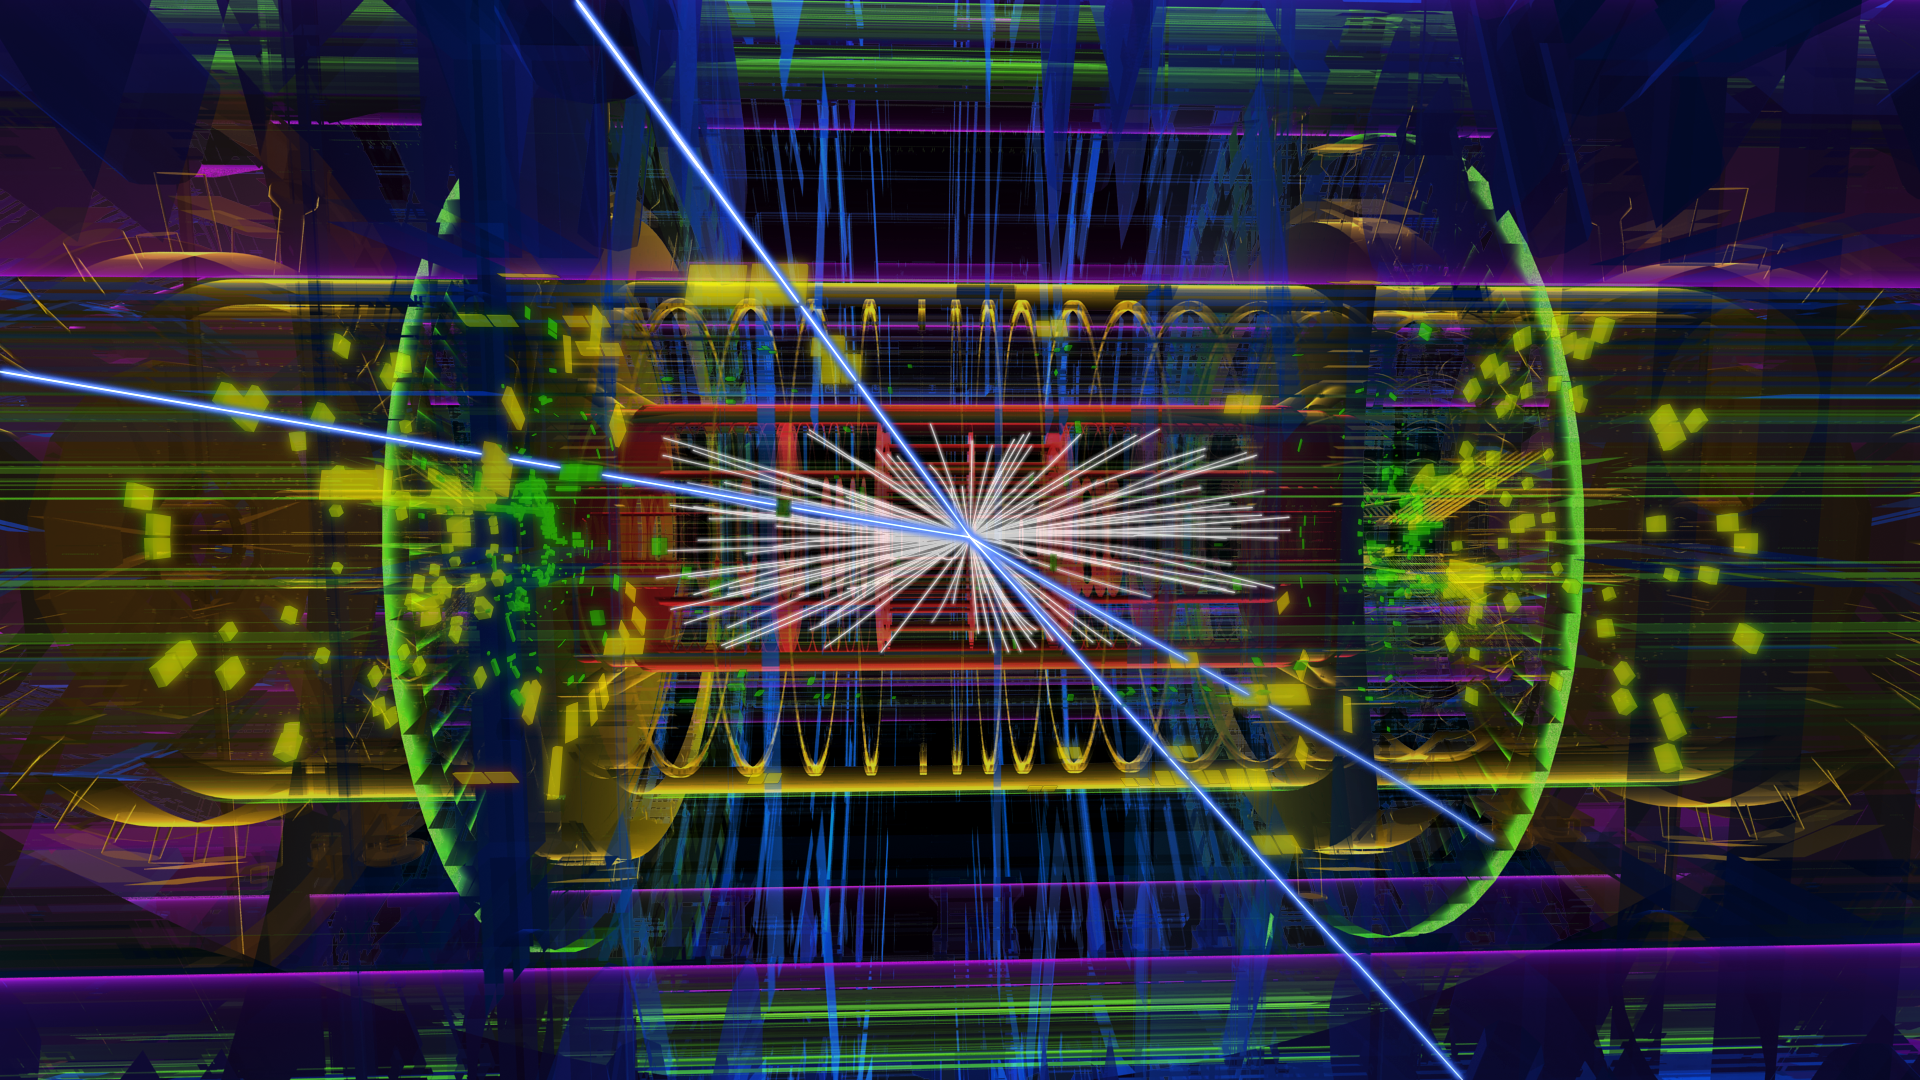
\includegraphics[width=0.5\textwidth]{figures/common_ana/Muon}
        \caption{        
            Event visualization of a four muon event in the ATLAS detector\cite{ATLAS:1697053}.
        }
        \label{fig:muon}
    \end{center}
\end{figure}

\subsection{Muon Reconstruction}
Reconstruction of muon is generally done in the following way: tracks are found in one part of the detector through pattern finding of hits in the ID/MS chambers. At least two matching segments from different subdetector parts are needed to form a track candidate. From the track candidate formed, global $\chi^{2}$ fits are done to add in other hits and drop outliers. While the main strategy of muon reconstruction is quite similar, different reconstruction strateties are used for muons in
different $P_{T}$ range and detector location to maximize reconstruction efficiencies. For details, see~\cite{muonReco2016}.

\begin{itemize}
\item \textbf{Combined muon(CB)}
    This strategy is optimal for the muons that are detected in both the ID and the MS. It applies for muons found in both the barrel and end-cap region of the detector. Tracks are each constructed from the ID and the MS. A global refit is done to remove outliers to improve the fit quality. This is mostly done by an outside-in approach where the tracks in MS are made to match the ones seen in the ID. Combined muons are also complemented by the inside-out muons: It looks for MS hits that can be associated with ID tracks and recovers muons that don't make it to the MS completely.

\item \textbf{Segment-tagged muons(ST)}
This method is used to identify lower $P_{T}$ muons that couldn't make it to multiple layers of the MS. If a track in the ID can be matched to at least one track segment in the MDT in the barrel or CSC in the end-cap, it will be selected as a segment-tagged muon. 

\item \textbf{Calorimeter-tagged muon(CT)}
This reconstruction method is used for even lower $P_{T}$ muons that could not make it to the MS at all. Muons between $15 GeV < P_{T} < 100GeV$ are formed from matching a track in ID with energy deposits in the calorimeter that matches the minimum-ionizing particle. This is optimized for barrel muons of $|\eta <0.1|$. 

\item \textbf{Extrapolated muon(ME)}
    This reconstruction strategy is designed for muons that are very forward and are swamped under noise from pile-up. Muon tracks in the MS chamber with a loose compatibility to the originating IP are ME muons are accepted as ME muons. This strategy extends the acceptance of muons in the forward region from $2.5<|\eta|<2.7$, as there is no ID coverage where they cannot be reconstructed by the above other methods.
\end{itemize}

\subsection{Muon Identification}
Muon identification is a set of selection criteria done on the candidate muons to cut out background from pions/kaon decays that would form muons that are not of interest to analyses. The identification increases the analysis signal sensitivity. In different analyses, depending on the signal type, different muon identification working points are used.

A couple of criteria are used for muon identification: $q/p_{significance}$, $\rho'$ and $\chi^{2}_{norm}$. They are defined as below~\cite{muonReco2016}:

\subsubsection*{Discrimination Criteria}
\begin{itemize}

\item \textbf{q/p significance}
    \begin{equation}
    q/p_{significance} = |(q/p)^{ID} - (q/p)^{MS}|/\sqrt{\sigma^{MS}_{P_{T}} + \sigma^{ID}_{P_{T}}}
    \end{equation}

This is the absolute value of the difference between the charges and the $P_{T}$ measurement divided by the sum of error in the $P_{T}$ measurement of both the ID and MS.

\item \textbf{$\rho'$}
    \begin{equation}
    \rho' = |P_{T}^{MS} - P_{T}^{ID}| / P_{T}^{Combined}
    \end{equation}

This is the absolute value of the difference between the $P_{T}$ of the MS and the ID divided by the combined $P_{T}$ of the muon candidate.

\item \textbf{$\chi_{norm}^{2}$}
    This is the $\chi^{2}$ of the fit from the combined muon track from both the ID and MS.

\end{itemize}

These selection criteria for the muon groups above result in five different working points.

\subsubsection*{Muon Working Points}
\begin{itemize}

\item \textbf{MEDIUM} \newline
This is the most commonly used working point. q/p significance $<$ 7. It accepts only the CB and IO muons.  

\item \textbf{LOOSE} \newline
    The loose working point accepts all the muons that pass the medium working point. It also accepts low-$P_{T}$ muons, including IO muons with $P_{T}$ lower than 7GeV. Some ST and CT muons are also accepted under certain circumstances~\cite{muonReco2016}

\item \textbf{TIGHT} \newline
    This working point accepts a subset of the medium working point muons. In addition, they are required to have a normalized $\chi^{2}$ of less than 8. The requirement on q/p compatibility and $\rho'$ depends on $\eta$ and $P_{T}$ of the muon.

\item \textbf{HIGH $P_{T}$} \newline
This working point only accept muons that also pass the medium working point requirement. Owing to their high $P_{T}$, the reconstruction can be done with the MS alone for a higher resolution.

\item \textbf{LOW $P_{T}$} \newline
The Low-$p_{T}$ working point includes all of the muons in the medium working point, it's identical to the medium working point muon set above $P_{T}=18GeV$. But this working point also includes muons with lower $P_{T}$ that does not make it to the middle of the MS, this working point includes muons down to 3 GeV. 

\end{itemize}

\begin{figure}[!htb]
    \begin{center}
        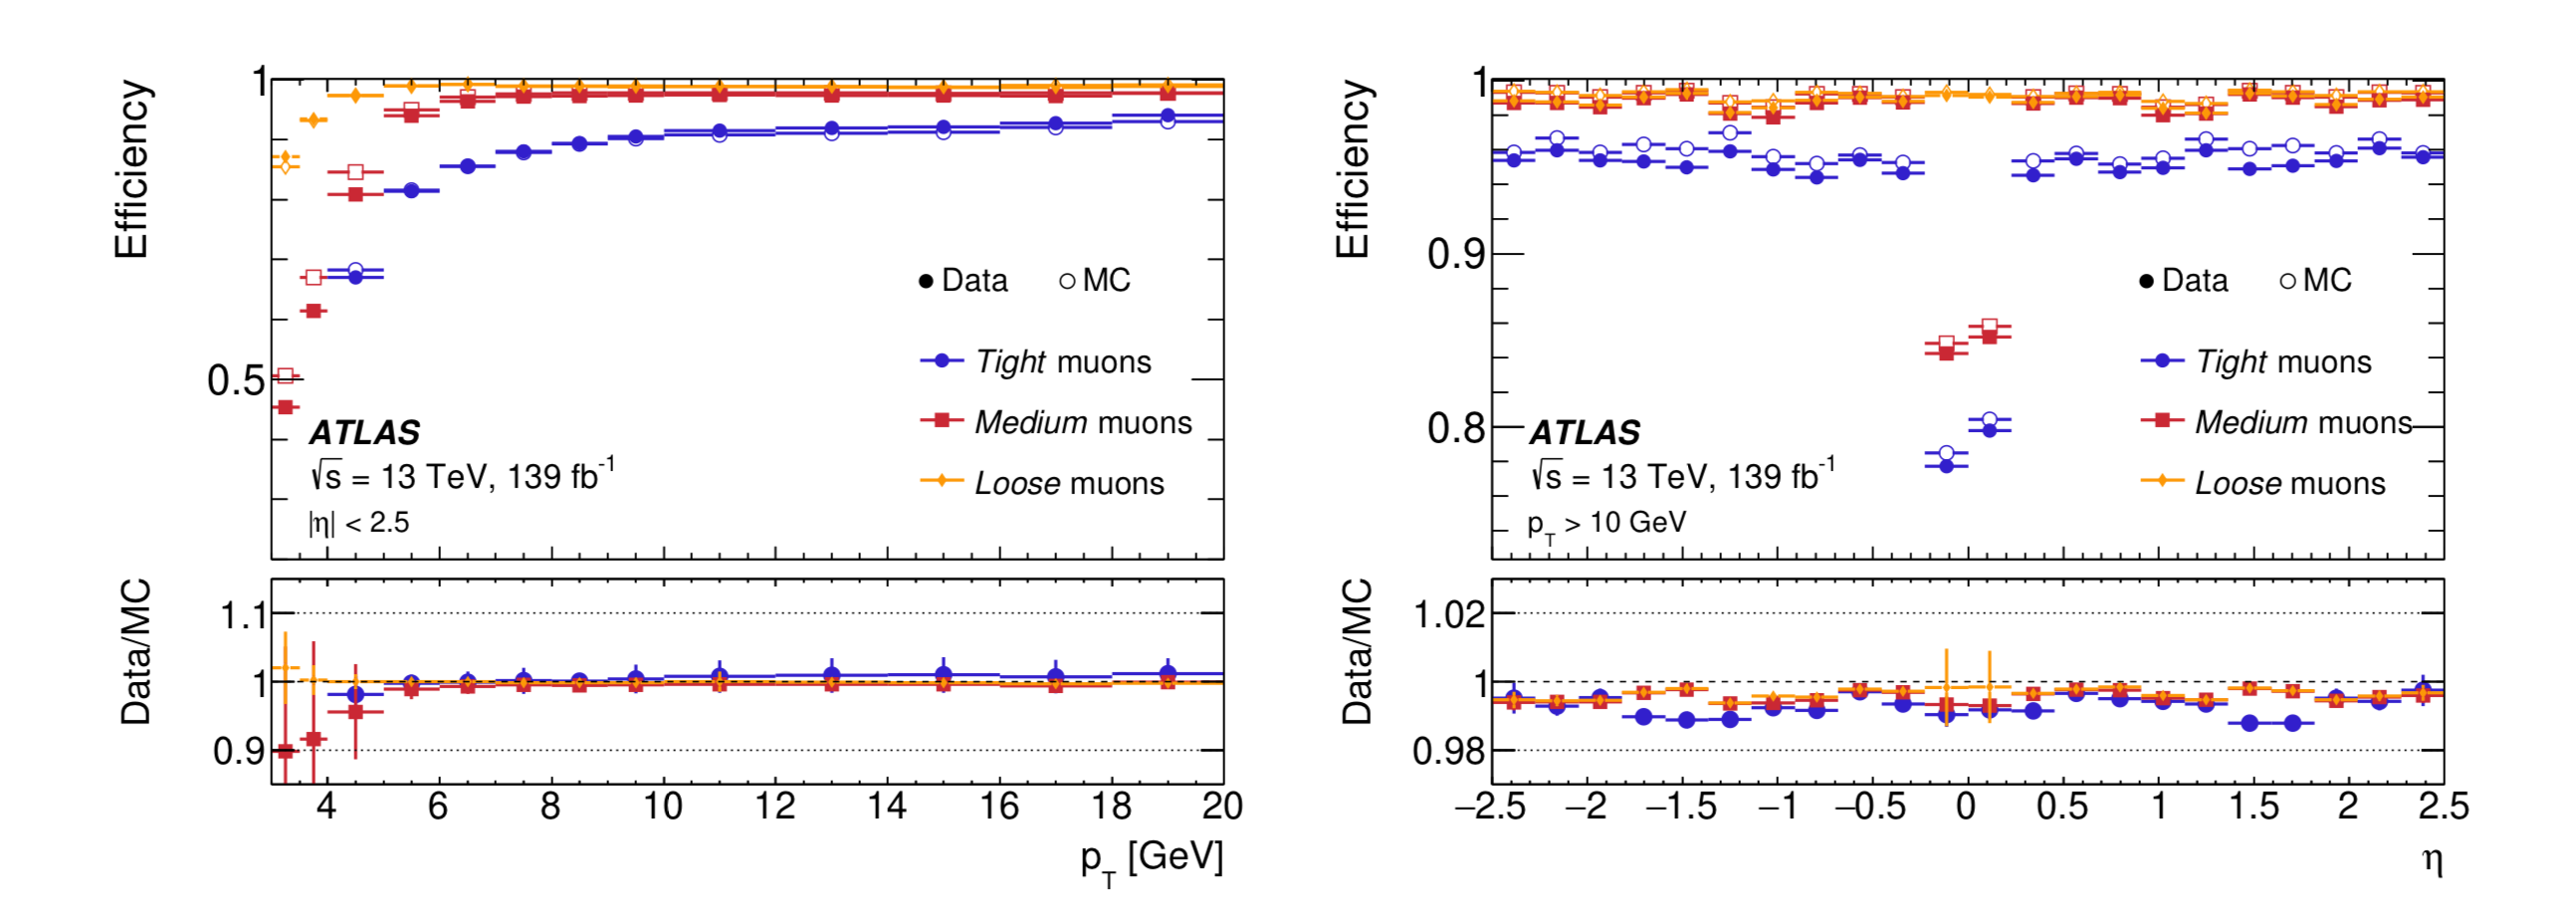
\includegraphics[width=1\textwidth]{figures/common_ana/IdentificationEff}
        \caption{
            This figure shows the reconstruction and identification efficiencies in different variable range in different working points\cite{Aad:2746302}.
        }
        \label{fig:isolationWP}
    \end{center}
\end{figure}



\subsection{Muon Isolation}
After the reconstruction and identification of the muon candidates, a set of muons are formed. The next step is to pick out muon candidates of interest from muon isolation. On ATLAS, the leptons of interest to physics analyses came from the hard primary vertex decay of radially decaying particles. W, Z, Higgs bosons or other BSM particles such as the Z' are examples decays that concern analyzers. Muons formed this way are known as the "prompt muons", they are usually clean and do not have many
associated neighboring hits. Less interesting muons came from the semileptonic decay from jet fragmentation, these muons decays are formed with lots of neighboring hits. From this difference, associated neighboring hits can be used as criteria to discriminate muons of interest from the muons not of interest. This step is called muon isolation. Signal sensitivity is cut down in the background and the search. Depending on the muon type, two different variables are used for muon isolation, one is the track-based isolation and other is calorimeter-based isolation.

\subsubsection*{Isolation Parameters}
The parameters used in the isolation criteria are defined as the following:
\begin{itemize}
    \item  $P_{T}^{varcone\:size}$ \newline
        The track-based isolation variable, $P_{T}^{varcone\:size}$ are the sum of the $P_{T}$ of all the tracks in a variable-sized cone. The variable-sized cone(varcone) is defined as below.

    
\begin{equation}
 \delta R = min(\frac{10}{P^{\mu}_{T}[GeV]}, \delta R_{max}) 
 \end{equation}

The term is $P_{T}$ dependent, the larger the $P_{T}$, the smaller the cone. 
    \item $E^{\textrm{topocone\:size}}_{T}$ \newline
        A calorimeter based parameter $E^{\textrm{topocone\:size}}_T$ is defined as the sum of the energy deposit in a $\delta R$ size topo cone. 

\end{itemize}

The isolation criteria using track-based variables is the variable that is related to the transverse momentum of the muon. Studies are done on data Monte Carlo to get the best cut-off point. The different working points are listed below in Figure~\ref{fig:isolationWP}.

%\begin{figure}[!htb]
%    \begin{center}
%        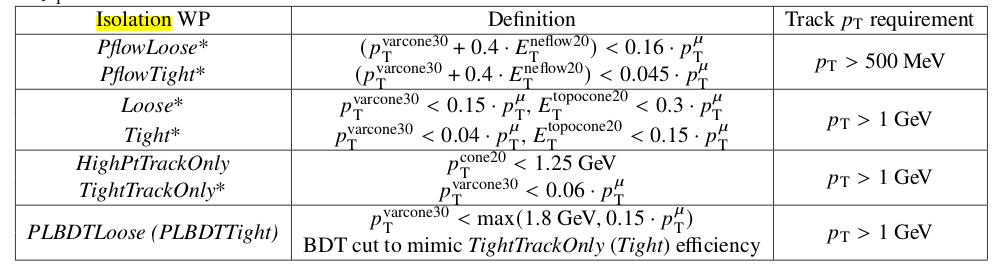
\includegraphics[width=0.75\textwidth]{figures/common_ana/Isolation}
%        \caption 
%        {
%            This figure shows the isolation working points on ATLAS from full run2~\cite{Aad:2746302}.
%        }
%        \label{fig:isolationWP}
%    \end{center}
%\end{figure}

\begin{figure}[!htb]
    \begin{center}
        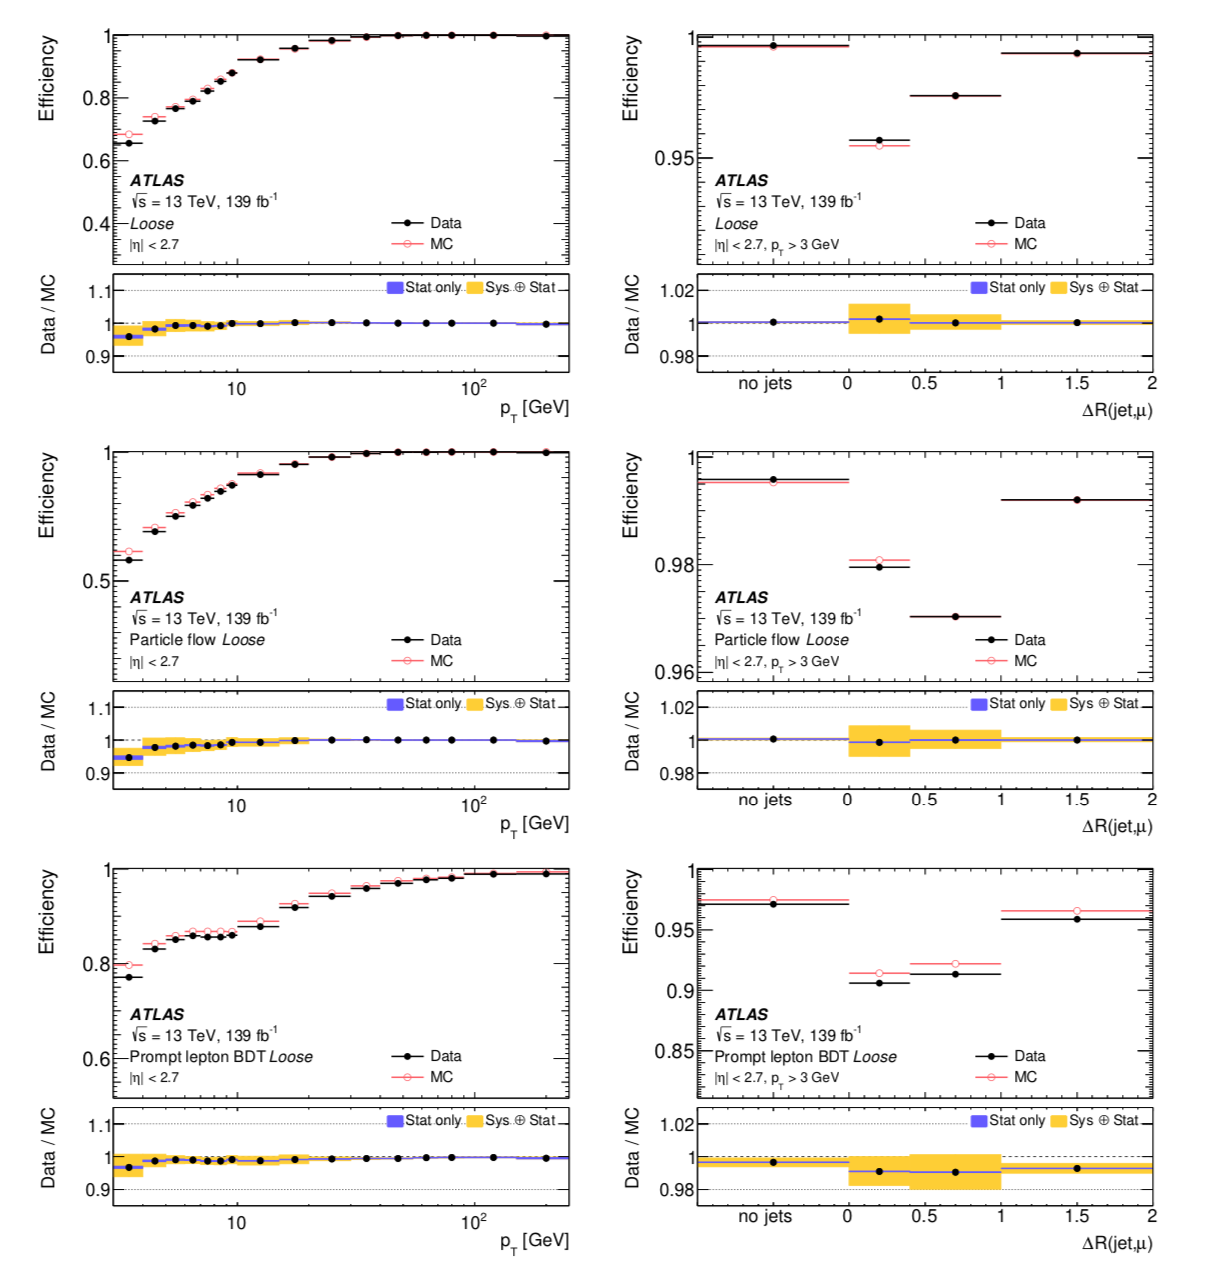
\includegraphics[width=0.75\textwidth]{figures/common_ana/IsolationEff1}
        %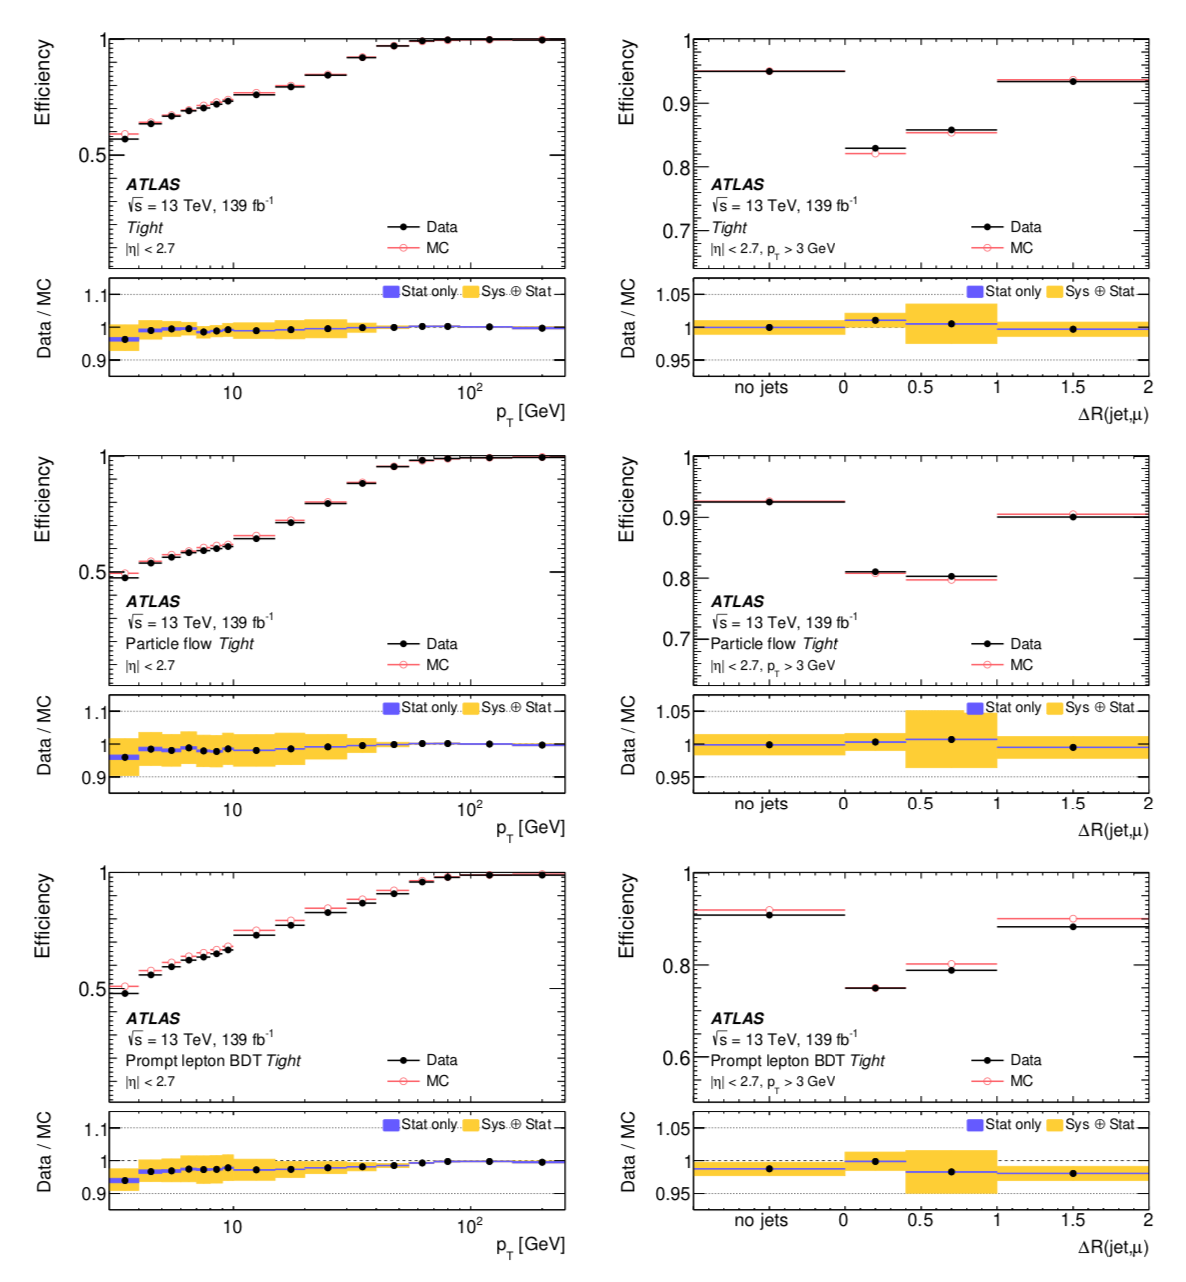
\includegraphics[width=0.75\textwidth]{figures/common_ana/IsolationEff2}
        \caption{
            This figure shows the isolation efficiency in different variable range in different working point\cite{Aad:2746302}.
        }
        \label{fig:isolationWP}
    \end{center}
\end{figure}

Different isolation working points are used for optimal sensitivity. 


\subsection{Muon Calibration}
Given the difference between imperfect Monte Carlo generation and data, a calibration factor is derived from comparing the MC to data using some known physics process $J/\Psi$ to $\mu \mu$ and Z to $\mu \mu$. The calibration is done on the $P_{T}$ of the muon. 
The calibration is dependent on the detector angle, and the formula is summarized as below, where the constants are derived from the data and simulation of the samples.

%In data there is always margin for calibration error, and monte carlo is also not necessarily accurately describing the experimental environment. To match data result to the actual physics process that happened, transverse momentum correction done on both the MS tracks muons and the ID track on the MC result as follows: 

\begin{equation}
P_{T}^{Cor,Det} = \frac{P^{MC, Det}_{T} + \sum_{n=0}^{1} S_{n}^{Det}{\eta, \phi}(P_{T}^{MC, Det})^n}{1+\sum_{m=0}^{2}\delta r_{m}^{Det}(\eta, \phi)(P_{T}^{MC, Det})^(m-1) g_{m}}
\label{eq:muoncalib}
\end{equation}

Here $P_{T}^{MC, Det}$ is the uncorrected transverse momentum, $g_m$ is a unit Gausssian distribution, $\delta r^{Det}_{m}(\eta, \phi)$ and $s_{n}^{Det}(\eta, \phi)$ are the momentum resolution smearing and scale correction resolution. 

The correction is then applied to the combined muon in the following way:

\begin{equation}
P_{T}^{Cor, CB} = f *P_{T}^{Cor, ID}+ (1-f) \cdot P_{T}^{Cor, MS}
\label{eq:muoncalibfactor}
\end{equation}

The weight f in the above is obtained from MC simulation. $P_T^{Cor, CB}$ and $P_T^{Cor,ID}$ are the corrected transverse momentum in CB and MS respectively.


%\begin{equation}
%\[\delta R = min( \frac{10}/P_{T}[GeV] , \delta R_{max} )\]
%\end{equation}



%For better discrimination effciency, in Run II, ATLAS has moved away from an iterative based method and moved towards a image algorithm for primary vertex finding. A brief description is as the
%following:  
%
%1. A three-dimensional binned box is first defined, the x and y dimension is 4 mm long and the z dimension is 400 mm, a 3-d histogram is made for this 3d box as input data. 
%
%2. Helical tracks are back-projected back to this histogram using a voxel ray-tracking algorithm. All the histogram in each bin crossed by a track is incremented by the path length of the linearized rack in that bin. an example back projected in shown 
%% Whats a vortex ray-tracing algorithm? 
%
%3. This projection is Fourier transformed into frequency sapce.
%
%4. A filter composed of both the angular accpetance of the ATLAS tracking detector in the fourier inverse of the angular acceptance and a four-term Blackman-Harris window filter is used to lessen the effect of high frequency variation is used to multiplied by the projection in the above step. 
%
%5. The filtered image is then transformed back to position space in x, y and z.  
%
%5. The resulting imag is passed to a clustering algorithm where the seeds are identified from the peaks. 

\section{Jets}
\label{sec:Jet}
Colored charge particles are govern by the strong force under the SM. This includes quarks and gluons. Under the strong force, when the distance is up to a certain value in an energy scale, the potential of these color charges would increases with distance apart. The increased potential leads to extra quark and gluon formation. The newly formed quark and gluons that are generated experiences a similar effect, which lead to further spliting from the original primary seed particle. This effect is known as parton showering. 
Showering lead to a cascade of energy deposits in the detector that does not look anything like the original particles. The jet algorithms aims to reverse reverse the process, it reconstructs for the physics properties of the the original primary quark/gluon from the resulting energy deposits. Figure~\ref{fig:jetEvent} is a visualization of an ATLAS event with two high $p_{T}$ jets.

The following is a schematic understanding of how jet finding is achieved. 

$\bullet$ \textbf{Jet showering}

Quark/gluon formed $\rightarrow$  Parton Showering $\rightarrow$ Detector Energy Deposit

$\bullet$ \textbf{Jet Reconstruction}

Energy Deposit on Detector  $\rightarrow$  Topo-cell Clustering $\rightarrow$  Topo-Clusers $\rightarrow$  Jet-Finding Algorithm $\rightarrow$ Jet


\begin{figure}[!htb]
    \begin{center}
        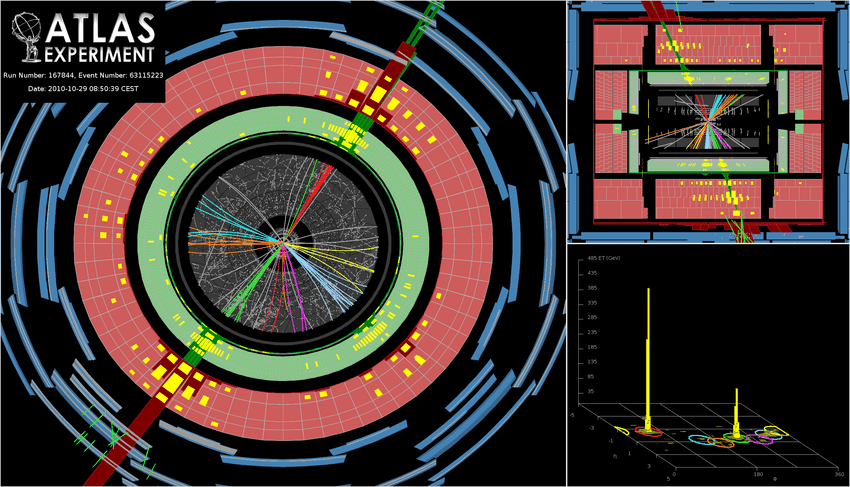
\includegraphics[width=0.7\textwidth]{figures/common_ana/JetEvent}
        \caption{        
            An simulation ATLAS event containing two high $p_{T}$ jet event~\cite{jetEvent}.
        }
        \label{fig:jetEvent}
    \end{center}
\end{figure}

% Why is there a topocell clustering algorithm before jet finding? Maybe it's due to the physics, each one looks like a potential quark/gluon candidate. 
% 
\subsection*{Topo-cell clustering}
\label{Topocell clustering}
This step clusters the lowest level calorimeter cells energy deposits into topological clusters. ATLAS uses a 3-D clustering algorithm. 

First, a seed cell with a high signal-to-noise(S/N) ratio above a certain level is found. Then, cells neighboring the seed cells in the 3-D that satifies certain lower threshold level are collected along with the seed cell to the topocluster. Lastly, a final set of cells that surround the second set of collected cells are added to the cluster. 

\subsection*{Jet Finding algorithm}
\label{sec:JetFinding}
% Add the C/A clustering algorithm
% Add the KT algorithm

Jet finding algorithm aims to merge the topoclusters from the previous step to form jets. An important feature for a jet finding algorithm is that it needs to be infra-red and collinear(IRC) safe. In an IRC safe algotihm, soft and small angle radiation addition to the jet will not change the constituent or calculation of the jet. This requirement avoids the divergence in probability calculations that would lead to infinities when jet splitting happens.

All of the main ATLAS jet finding algorithms make use of the following quantities:

\begin{equation}
    d_{ij} = min(k_{ti}^{2p}, k_{tj}^{2p}) \frac{\Delta^{2}}{R^{2}}
    \label{sec:topo}
\end{equation}

\begin{equation}
    d_{iB} = k^{2p}_{ti}
\end{equation}

Here, $\Delta_{ij}^{2} = (y_{i}- y_{j})^2 + (\phi_{i} - \phi_{j})$, $k_{ti}
$, $y_{i}$, and $\phi_{i}$ are the transverse momentum, rapidity and azimuth angle of particle i. p is a parameter on the energy scale~\cite{HEP2008}. $d_{ij}$ and $d_{iB}$ quantity are the distance between particle i and j and distance between i and B respectively. 

The algorithm clusters the topoclusters with the smallest distance together~\ref{sec:topo}, until no clusters are left. p is taken to be -1 for the anti-KT jet finding algorithm; 1 for the KT algorithm and 0 for C/A. 

The current ATLAS standard jet finding algorithm is the Anti-KT algorithm.

\subsection{Jet calibration}
After jets are formed, they need to be calibrated to reflect the direction, momentum and energy of the originated quarks or gluons. The jets are required to be calibrated. In ATLAS, jets energy is measured out in both the EM calorimeter and the hadronic calorimeter, the topoclusters are calibrated to the EM scale, but not the hardronic scale. Jet energy correction needs to be perfored before the object can be used for analysis. The jet calibration takes the following steps as
shown in Figure~\ref{fig:JetCalibration}.

\begin{figure}[!htb]
    \begin{center}
        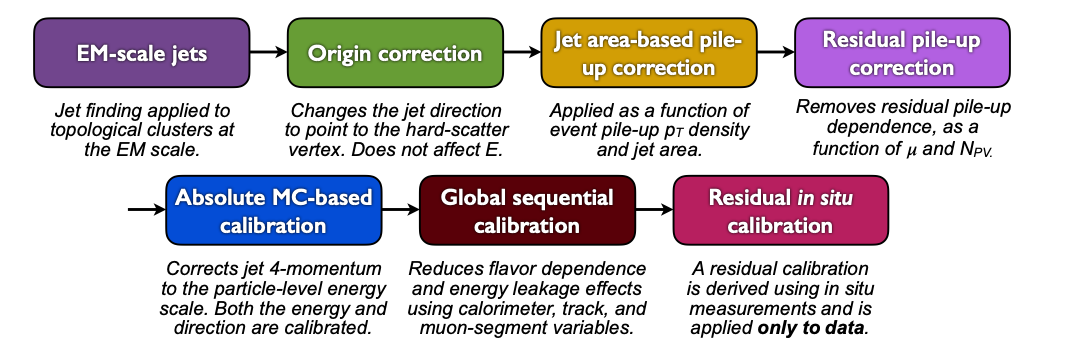
\includegraphics[width=1.1\textwidth]{figures/common_ana/JetCalibration}
        \caption{        
            The steps of calibration the jet object under take before analyzable objects\cite{Mehlhase:2770815}.
        }
        \label{fig:JetCalibration}
    \end{center}
\end{figure}

\section{Photon}
\label{sec:Photon}
Photons on ATLAS are reconstructed from clusters in the EM Calorimeter sometimes paired with tracks in the tracker. Photons and electrons shares a similar reconstruction algorithm. Like muons and jets, photons are first reconstructed, identified, isolated and lastly calibrated before being used for analysis. 

\begin{figure}[!htb]
    \begin{center}
        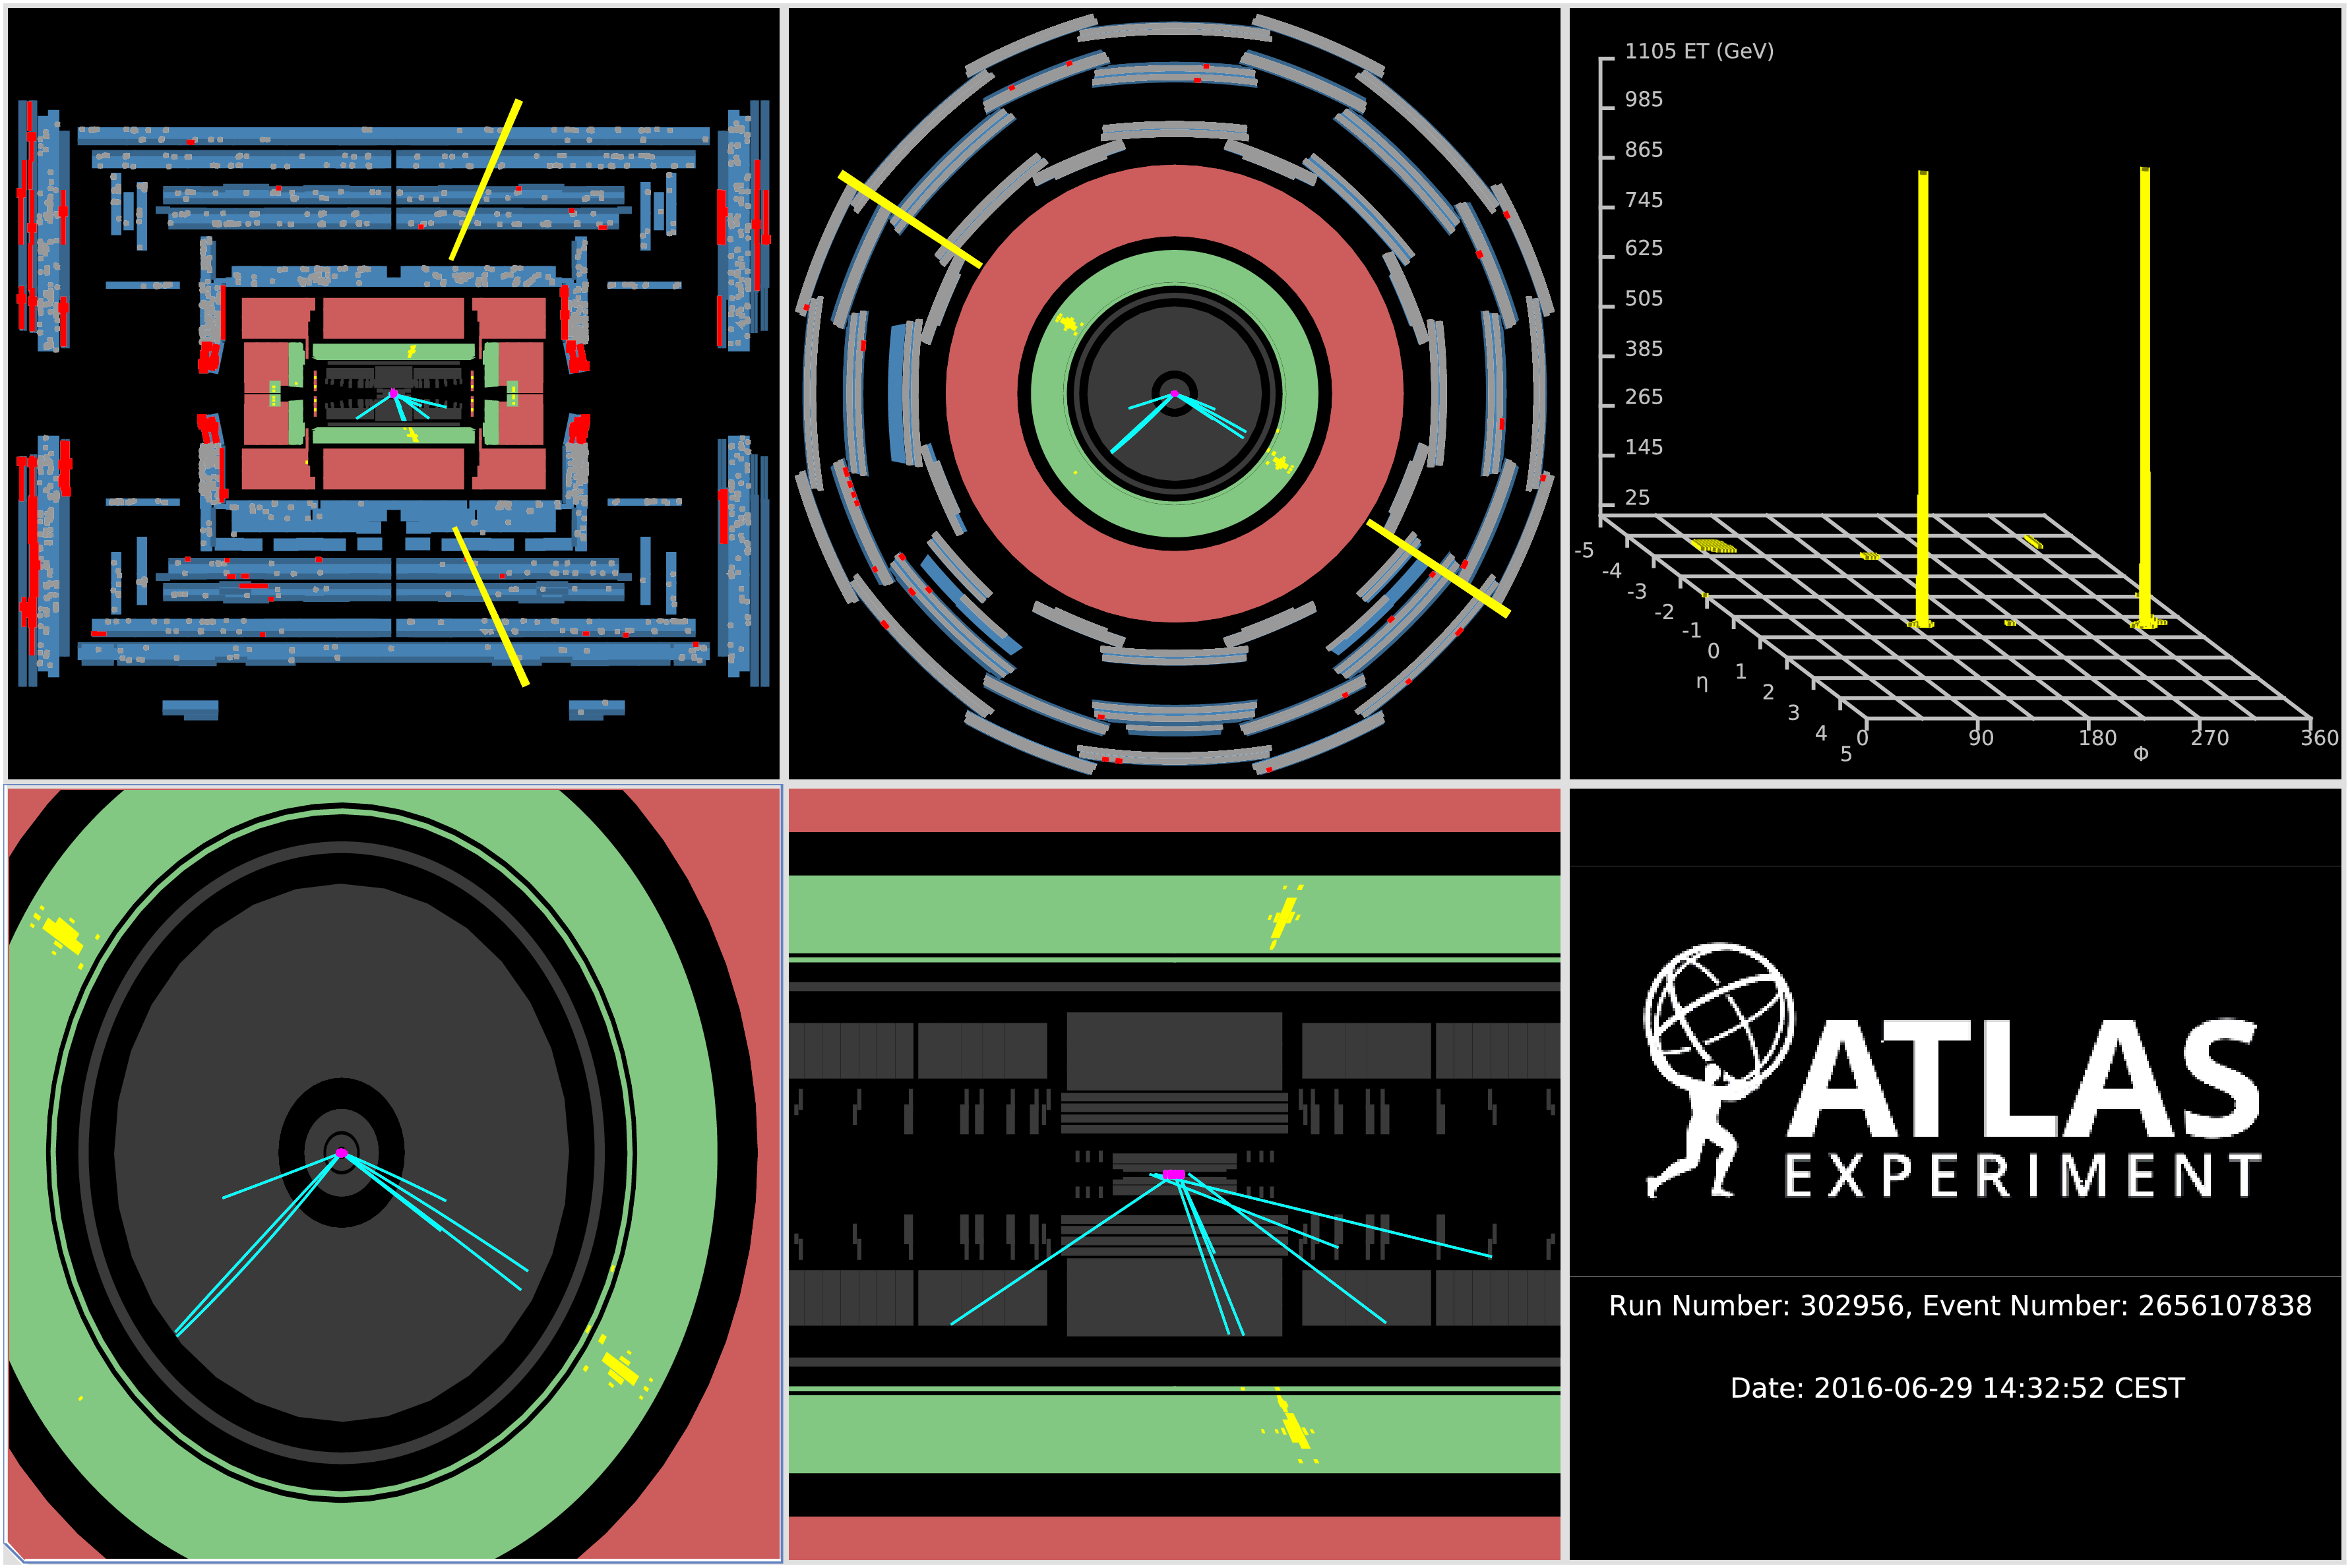
\includegraphics[width=0.7\textwidth]{figures/common_ana/photonEvent}
        \caption{        
        An ATLAS event display that contain two photons~\cite{atlas}.
        }
        \label{fig:photonEvent}
    \end{center}
\end{figure}

\subsection{Photon Reconstructionn}
Photons interact with the active material in the EM calorimeter. They shower and leave deposits in there. The first step to photon reconstruction is the finding of clustering seed. A sliding window of $\delta \eta \times \delta \phi = 0.025 \times 0.0245$ is used to scan for a clustering seed with energy deposit above 2.5 GeV. Neighboring hits are added to the seed to form a cluster through the clustering algorithm~\cite{Lampl:1099735}. 
These cluster are matched by tracks in the inner detector, these tracks are used for vertex construction. If no vertex or tracks are matched, they are unconverted photons, otherwise, they are considered converted photons. Converted photons are photons that originates from electrons. 

%\begin{figure}[!htb]
%    \begin{center}
%        \includegraphics[width=1.1\textwidth]{figures/common_ana/MuonReconstruction}
%        \caption{        
%            Schematics showing the window used to scan the EM Calorimeter for clustering seeds~\cite{gammaCalibration2019}.
%        }
%        \label{fig:MuonReconstruction}
%    \end{center}
%\end{figure}

\subsection{Photon Identification}
Like muons, not all photons candidates are photons in the primary processes. Some came from non-prompt photons from decaying jets. Photon identification utilizes kinematic cuts from calorimeters variables to separate the prompt photons from the fake photons from jets~\cite{gammaCalibration2019}.
There are two photon working points, the loose working point uses information from the shower shape in the calorimeter. The tight working point uses information from the calorimeter strips and has different requirements for uncoverted and converted photon for optimal classfication power. Details can be found in~\cite{gammaCalibration2019}. 

\subsection{Photon Isolation}
Photon isolation is a strategy that is effective in identifying the prompt photons from the non-prompt photons that are produced in association with other product. The isolation is a cut on the transverse energy or transverse momeumtum for a certain $\delta R $ cone size around the photon candidate. The isolation variable for the calorimeter and tracker are calculated separately~\cite{gammaCalibration2019}.

%\begin{itemize}
%
%\item LOOSE \newline
%\begin{equation}
%    E_{T}^{iso}|_{\Delta R < 0.2} < 0.065 \times E_{T}
%\end{equation}
%and 
%\begin{equation}
%    p_{T}^{iso}|_{\Delta R<0.2}<0.05\times E_{T}
%\end{equation}
%
%\item TIGHT \newline
%\begin{equation}
%    E_{T}^{iso}|_{\Delta R<0.4} <0.022 \times 0.022+ 2.45 GeV
%\end{equation}
%and 
%\begin{equation}
%    p_{T}^{iso}|_{\Delta R<0.2 }< 0.05 \times E_{T}
%\end{equation}

%\end{itemize}

\subsection{Photon Calibration}
Photons in ATLAS takes the following steps to be calibrated. 
First, the photon energy is estimated from the deposits in the calorimeter by a multivariate regression algorithm on the detector material in simulation. Later, correction is then done on the energy scale in the different layers of the EM calorimeter from Higgs to $\mu \mu$ data. After that, geometric correction is done on the data to correct for the non-uniformity in the detector in the boundaries of the calorimeter modules. Lastly, an overall adjustment on the energy scale is done in the data~\cite{gammaCalibration2019}.

